\documentclass{beamer}
\usetheme{Darmstadt}
\usecolortheme{orchid}

\useoutertheme{infolines} % infolines, miniframes, shadow, sidebar, smoothbars, smoothtree, split, tree
\useinnertheme{rectangles} % rectangles, circles, inmargin, rounded

\setbeamertemplate{blocks}[rounded][shadow=true]

% suppress navigation bar
\beamertemplatenavigationsymbolsempty

% Additional packages
\usepackage{color}
\usepackage{graphicx}
\usepackage{listings}

\usebeamercolor{block title}
\colorlet{code}{bg}
\usebeamercolor{block title alerted}
\colorlet{keyword}{bg}

\lstdefinestyle{custom_python}{
	language=Python,
	basicstyle=\color{code}\ttfamily\scriptsize,
	breaklines=true,
	frame=single,
	keywordstyle=\color{keyword}\ttfamily\scriptsize,
	otherkeywords={POINTER, self}
}


\title[Practical Course]{Practical Course in Bioinformatics}
\subtitle{Algorithm Group -- Final Presentation}
\author[Berrendorf, Raissi, Lange, Voit]{Max Berrendorf \and Thomas Lange \and Tina Raissi \and Matthias Voit}
\institute[]{ZKF Research Group Computational Biology and Bioinformatics\\
	Helmholtz Institute for Biomedical Engineering\\
	RWTH University Hospital
}
\date{}

\AtBeginSection{
	\frame{
		\sectionpage
	}
}

\begin{document}
% ========================== BEGIN TITLE PAGE =========================== %
\frame{\titlepage}

% ============================= BEGIN TOC ============================= %
\begin{frame}
    \frametitle{Outline}
    \setcounter{tocdepth}{1}
    \tableofcontents[]
\end{frame}
% ============================== END TOC ============================== %
\section{Outsourcing computation to C}
\begin{frame}%[allowframebreaks]
	\frametitle{Outsourcing computation to C}
\end{frame}

\section{Minimising Deepcopies}
\begin{frame}%[allowframebreaks]
	\frametitle{Minimising deepcopies}
\end{frame}

\section{Results}
\begin{frame}[plain]
	\frametitle{Jaccard Test}
	\begin{center}
		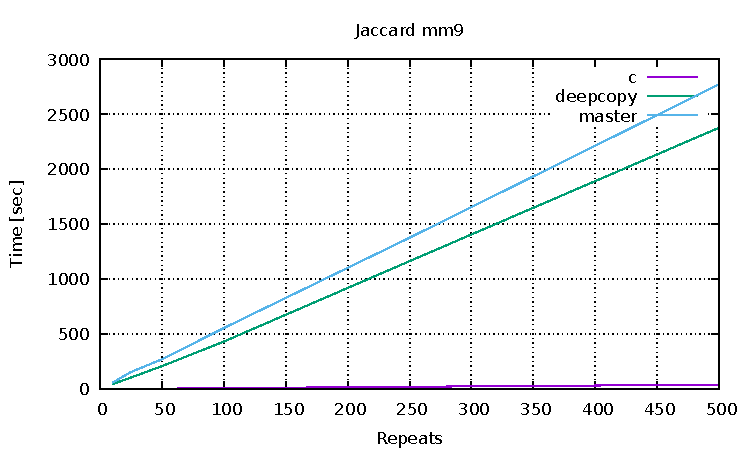
\includegraphics[width=1.0\textwidth]{img/jaccard-mm9}
	\end{center}
\end{frame}

\begin{frame}
	\frametitle{The End}
	\vfill
	\begin{center}
		Thank you for your attention!
	\end{center}
	\vfill
\end{frame}

\end{document}